\subsection{From plasma to grid: power flow and influences}\label{sec:powerflow}
The heat balance above is derived as a chain of formulas. Figure~\ref{fig:powerflow} shows the same numbers as a
flow: the width of each band is proportional to the power. Below the nodes are the parameters that set each value.
An interactive version, in which every node and every parameter can be clicked, exists as a web page; the figure
is produced by \texttt{stellarator/einflussgraph.py}.

\begin{figure}[H]\centering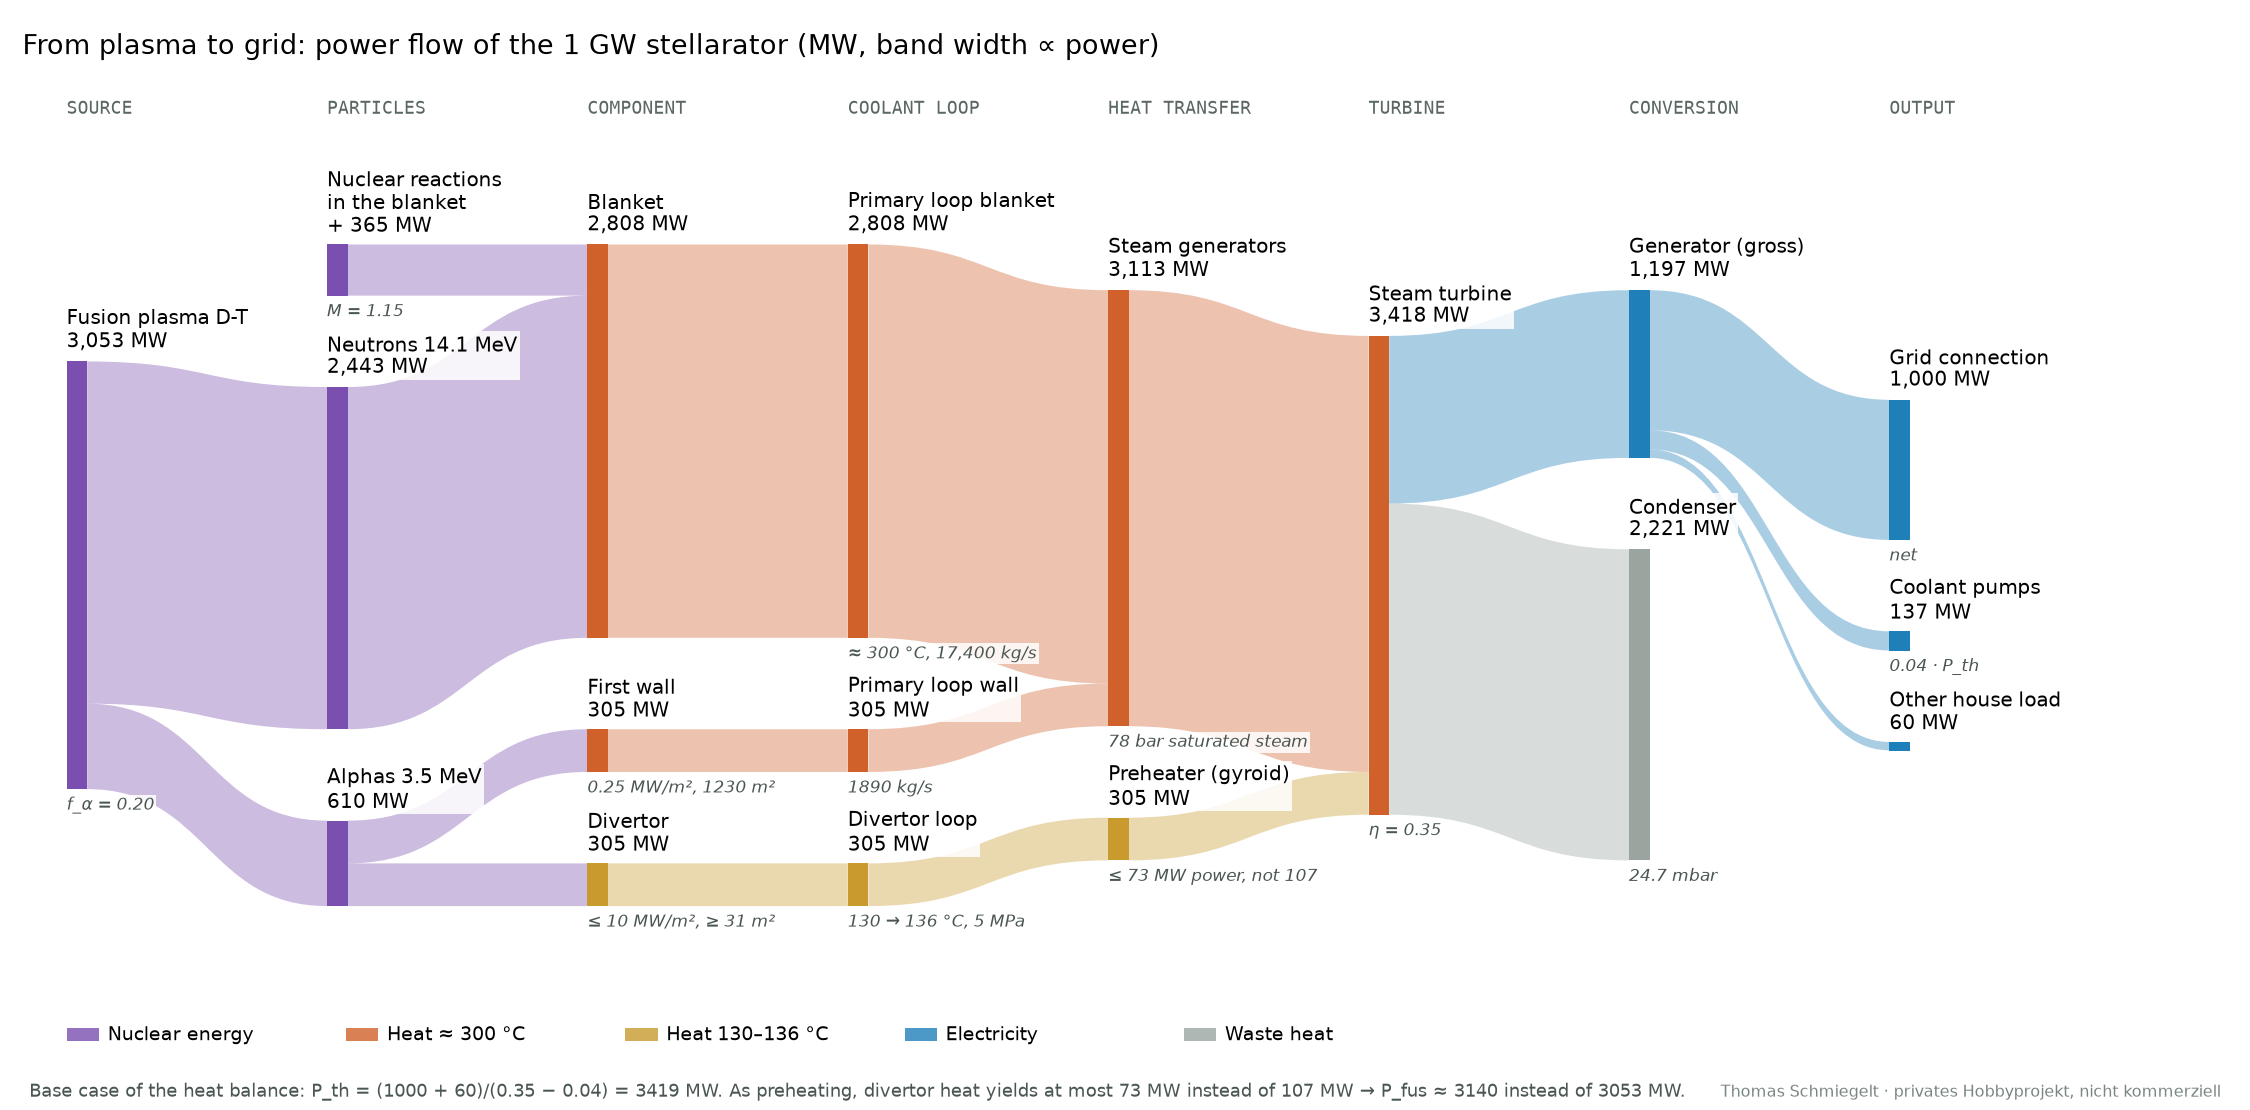
\includegraphics[width=\linewidth]{bilder/einflussgraph_en.png}
\caption{Power flow from the fusion plasma to the grid connection (base case of the heat balance, MW).}\label{fig:powerflow}
\end{figure}

\paragraph{How to read it.} Of \SI{3053}{MW} fusion power, \SI{1000}{MW} reach the grid, just under one third. The
largest loss is not in the plasma and magnet part of the plant but in the turbine: the condenser rejects
\SI{2223}{MW} as waste heat. This is true of every steam plant and follows from the live-steam temperature. The
chain has three places where the design directly affects the efficiency:
\begin{itemize}
\item the \textbf{coolant temperature} of blanket and wall (about \SI{300}{\celsius}). It sets the live-steam
  pressure of \SI{78}{bar} and thus $\eta=0.35$;
\item the \textbf{divertor temperature} (\SI{136}{\celsius}). It turns \SI{305}{MW} of heat into preheating only,
  which yields at most \SI{73}{MW} of electricity (Section~\ref{sec:preheater});
\item the \textbf{pressure losses} in channels and exchangers. Through the pumps (\SI{137}{MW}) they come directly
  off the net output.
\end{itemize}
The physics parameters ($f_\alpha$, $M$) determine how much fusion power is needed for \SI{1}{GW} net, not the
efficiency downstream.

\IfFileExists{components_en.tex}{\subsection{The components of the chain}\label{sec:components}
This section explains the components from the plasma to the grid in plain words. General background is referenced; numbers marked ``project'' are assumptions or results of this design.

\paragraph{1. Fusion plasma and magnet coils.} In the plasma, deuterium and tritium (D-T) fuse at about 150 million \si{\celsius} \cite{bt_iter_fusion}. Gas this hot touches no wall. Magnetic fields hold it in suspension. A stellarator shapes this field with twisted external coils alone and drives no current through the plasma. It therefore runs steadily by nature, but needs stronger magnets than a tokamak \cite{bt_stellarator}. Large machines such as Wendelstein~7-X use superconducting coils cooled to about \SI{4}{K} with liquid helium \cite{bt_w7x_en}. This needs a cryogenic plant. Project: the plasma delivers $P_\text{fus} = \SI{3053}{MW}$ (about \SI{3140}{MW} with the preheater correction). Open: the forces between the coils are about 1000 times those of W7-X, and the support structure is not solved yet.

\paragraph{2. Neutrons and alpha particles.} Each D-T fusion releases \SI{17.6}{MeV}. The neutron carries about \SI{80}{\percent}; the helium nucleus (alpha particle) carries the rest \cite{bt_dtfusion,bt_fusionpower}. The neutron has no charge. It leaves the magnetic field and deposits its energy in the wall and the blanket. The alpha particle stays in the plasma and heats it \cite{bt_tokamak}. Project: $f_\alpha = 0.2$ (exactly $3.52/17.59$). Assumption: the alpha power leaves the plasma half as radiation onto the first wall and half as a particle stream onto the divertor ($f_\text{div} = 0.5$). This split is open; it depends on the real plasma.

\paragraph{3. First wall.} The first wall is the lining that faces the plasma. It protects the coils and catches heat and radiation \cite{bt_firstwall}. At ITER it sits on detachable panels, and the armour changes from beryllium to tungsten \cite{bt_iter_blanket}. Tungsten has the highest melting point of all metals, but it is brittle \cite{bt_firstwall}. Project: the wall takes \SI{305}{MW} of radiation. That is \SI{0.25}{MW/m^2} on \SI{1230}{m^2}. The cooling channels are designed for \SI{0.5}{MW/m^2}, a factor of 2 in reserve. The cooling water (\SI{1890}{kg/s}) warms by \SI{30}{K}. Open: neutron damage to the wall material, which is not studied here.

\paragraph{4. Blanket.} The blanket sits behind the first wall. It has three jobs: it slows the neutrons and turns their energy into heat; it breeds tritium when neutrons hit lithium; and it shields the coils \cite{bt_breeding,bt_iter_blanket}. Tritium hardly exists in nature, and only the blanket can supply it \cite{bt_breeding}. Lead or beryllium multiply the neutrons (multiplication) \cite{bt_breeding}. Project: $M = 1.15$ (assumption). The blanket removes \SI{2808}{MW} with \SI{17400}{kg/s} of pressurised water at about \SI{300}{\celsius} and $\Delta T = \SI{30}{K}$. The EU-DEMO concept WCLL (water, lead-lithium) aims at these conditions \cite{arena2023}. Open: can the blanket remove \SI{2.8}{GW} and breed enough tritium at the same time?

\paragraph{5. Divertor.} The divertor guides particles and heat that escape the plasma along open field lines onto dedicated plates \cite{bt_divertor}. It removes ash and impurities and keeps the plasma clean \cite{bt_iter_divertor}. The ash consists mainly of helium, which D-T fusion produces \cite{bt_dtfusion}; vacuum pumps remove it. At the ITER divertor the heat load is steadily about \SI{10}{MW/m^2}, with slow peaks up to \SI{20}{MW/m^2} \cite{bt_iter_divertor}. Project: \SI{305}{MW} on at least \SI{31}{m^2} at \SI{10}{MW/m^2}. It is cooled cold (water \SI{130}{\celsius} in, \SI{136}{\celsius} out, \SI{5}{MPa}), as in EU-DEMO \cite{you2022}. The project assumes a copper alloy for this. Open: the lifetime under this load.

\paragraph{6. Primary cooling circuits.} The cooling circuits of blanket and wall carry the heat out. They use pressurised water, as in a pressurised-water reactor. The high pressure keeps the water liquid although it is far above \SI{100}{\celsius} \cite{bt_pwr}. Project: about \SI{300}{\celsius}, $\Delta T = \SI{30}{K}$, \SI{17400}{kg/s} through the blanket and \SI{1890}{kg/s} through the wall. The pressure of about \SI{16}{MPa} is an assumption. Choosing these conditions is also a project decision: it allows a turbine from a pressurised-water reactor. Open: the pipes must pass through the narrow coil gaps. The calculation shows ample room (more than a factor of 10 in reserve).

\paragraph{7. Steam generator.} The steam generator is a heat exchanger. Hot primary water flows through many thin tubes; on the outside, secondary-loop water boils into steam \cite{bt_steamgen}. The tube walls separate the loops, so primary water does not reach the turbine \cite{bt_steamgen,bt_pwr}. The project assumes that the primary water may carry tritium or activation products. Project: live steam at \SI{78}{bar}, saturated, \SI{2443}{kg/s}. These are the EPR values \cite{epr_en}. The steam is saturated, as in a pressurised-water reactor; the project assumes $\eta = 0.35$ for it. Open: tritium may migrate through the tube wall; this is not studied.

\paragraph{8. Divertor preheater.} The divertor heat arrives at only about \SI{130}{\celsius}. That is too cold for steam, but fine for preheating feedwater. This saves extraction steam, which then does work in the turbine. Project: the gyroid exchanger, a printed wall with winding channels, is to transfer the \SI{305}{MW}. Result of the calculation: the preheater yields at most \SI{73}{MW} of electricity, and only without temperature approach and without pumps. For comparison, \SI{107}{MW} would be \SI{35}{\percent} of \SI{305}{MW}. If the heat is lost entirely, the required fusion power rises by \SI{10}{\percent}. Open: the correlations come from small-scale experiments.

\paragraph{9. Steam turbine.} The turbine lets the steam expand in many stages and turns pressure into rotation \cite{bt_turbine}. With reheat, the steam returns to a heater after the high-pressure section and then flows on. This yields more work and fewer droplets on the last blades \cite{bt_turbine}. Project: heat $P_\text{th} = \SI{3419}{MW}$, efficiency $\eta = 0.35$, so \SI{1197}{MW} gross. For comparison, Isar~2 had \SI{3950}{MW} thermal and \SI{1485}{MW} gross; a turbine of this class suffices. Assumption: such a turbine is available. Open: whether a decommissioned turbine can be had.

\paragraph{10. Condenser and cooling tower.} The condenser cools the exhaust steam back into water. It works below atmospheric pressure so that the turbine extracts more energy \cite{bt_condenser}. The heat released must go somewhere: a wet cooling tower dumps it by evaporating part of the water \cite{bt_cooling}. Project: \SI{2223}{MW} of waste heat at \SI{24.7}{mbar} (\SI{20.9}{\celsius}). That is almost twice the electrical output, as in every steam power plant. Open: site and water demand of the cooling tower; the project has not determined them.

\paragraph{11. Generator.} The generator turns the rotation of the turbine shaft into electricity. It uses electromagnetic induction: a moving magnetic field induces a voltage in windings \cite{bt_generator}. Power plants use synchronous generators, which must run in step with the grid \cite{bt_generator,bt_turbine}. Project: it produces \SI{1197}{MW} gross of alternating current. Of this, \SI{197}{MW} go to the plant's own demand. The balance uses only the overall efficiency $\eta$; there is no separate generator efficiency in it. Open: selection and size.

\paragraph{12. Plant's own demand.} The plant uses part of its electricity itself. Project: the coolant pumps need \SI{137}{MW} ($0.04\,P_\text{th}$, assumption). A further \SI{60}{MW} covers the rest: the coil cryogenic plant, the tritium plant and buildings. The cryogenic plant keeps the coils at a few kelvin \cite{bt_w7x_en}. The tritium plant is to recover tritium from the blanket and exhaust gas and feed it back to the plasma (project description, not referenced). The value for the rest is an assumption; for the first-wall channels alone the project finds only about \SI{8}{MW} of pumping power. Open: the total of \SI{197}{MW} is not built up from single items.

\paragraph{13. Transformer and grid connection.} A transformer raises the generator voltage. At high voltage the same power needs less current, and the lines lose less heat \cite{bt_transformer}. The high-voltage grid then takes the power. Project: \SI{1000}{MW} net go to the grid. This is the target from which the whole chain was computed backwards. Transformer losses are not included in the balance. Open: grid connection point and design.
}{}
